% Latex source for:
%   "Rapid 3D inversion of gravity and gravity gradient data to test geologic
%    hypotheses" by Leonardo Uieda and Valeria C F Barbosa

\RequirePackage{fix-cm}
\documentclass[twocolumn,final]{svjour3}
%\documentclass[twocolumn,draft]{svjour3}
%\documentclass[twocolumn,referee]{svjour3}

\smartqed  % flush right qed marks, e.g. at end of proof

\usepackage{graphicx}
\usepackage{amsmath}
\usepackage[round,sort]{natbib}

% Custom commands
\newcommand{\vect}[1]{\mathbf{#1}}
\newcommand{\mat}[1]{\mathbf{#1}}

\journalname{International Association of Geodesy Symposia}

\begin{document}

% TITLE AND AUTHORS
%%%%%%%%%%%%%%%%%%%%%%%%%%%%%%%%%%%%%%%%%%%%%%%%%%%%%%%%%%%%%%%%%%%%%%%%%%%%%%%%
\title{
    Rapid 3D inversion
    of gravity data
    to test geologic hypotheses
}
\author{Leonardo Uieda \and Val\'eria C. F. Barbosa}

%\titlerunning{Short form of title}        % if too long for running head
%\authorrunning{Short form of author list} % if too long for running head

\institute{
    L. Uieda \and V.C.F. Barbosa \at
        Observat\'orio Nacional,
        Rua General Jos\'e Cristino 77,
        20921-400 Rio de Janeiro - RJ, Brazil.
        \email{leouieda@gmail.com; valcris@on.br}
}

\date{Received:  / Accepted: }

\maketitle

% ABSTRACT AND KEYWORDS
%%%%%%%%%%%%%%%%%%%%%%%%%%%%%%%%%%%%%%%%%%%%%%%%%%%%%%%%%%%%%%%%%%%%%%%%%%%%%%%%
\begin{abstract}
% Note: Max 250 words
Meh


\keywords{
    Gravity inversion \and
    Gravity gradiometry \and
    Modeling \and
    3D \and
    GOCE
}
\end{abstract}

% INTRODUCTION
%%%%%%%%%%%%%%%%%%%%%%%%%%%%%%%%%%%%%%%%%%%%%%%%%%%%%%%%%%%%%%%%%%%%%%%%%%%%%%%%
\section{Introduction}

\begin{sloppypar}
Forward modeling of potential fields
is a useful way to generate geophysical models
that incorporate the interpreter's knowledge
about the regional and local geology.
However,
when modeling in 3D
and/or trying to fit multiple data components
(e.g., in gravity gradiometry),
forward modeling can be a tedious task.
That is because the interpreter is
tasked with simultaneously
constructing geologically realistic models
and supervising the data fit.
\\\indent
These problems are partially solved
by methods of geophysical inversion,
which automatically fit the data.
Conversely,
inverse problems introduce other challenges of their own.
Most geophysical inverse problems are ill-posed
because their solutions are neither unique nor stable.
Thus, they require the introduction of prior information,
usually through regularization \citep{silva_potinversion}.
Moreover, 3D inverse problems are computationally expensive.
\\\indent
Recent developments in potential field inversion
have proposed different types of regularization
to transform the ill-posed problem into a well-posed one
\citep[e.g.,][]{last_kubik, li_oldenburg, zhdanov_focusing, silva_interactive,
silvadias_adaptive, martins_tv}.
In addition,
several techniques have been applied
to overcome the computational complexity,
like data compression \citep{zhdanov_compression, li_compression},
lazy evaluation of the sensitivity matrix \citep{uieda_planting},
moving footprint \citep{cox_footprint},
and parallel computation \citep{cuma_largescale}.
\\\indent
We call attention
to the method called ``planting anomalous densities''
of \citet{uieda_planting}
that has been further developed by \citet{uieda_shape}.
This method is based on
the work of \citet{rene}.
It uses an iterative algorithm
to automatically grow the anomalous bodies
around user-specified prismatic elements called ``seeds'',
which have fixed density contrasts and positions.
Thus, the seeds provide
a skeletal outline of the presumed geologic bodies.
The inversion algorithm concentrates mass
around this ``skeleton''
in a way that both
fits the observed data
and yields compact bodies.
Therefore,
these seeds provide
a way for the interpreter
to impose prior geologic and geophysical information
on the inversion.
The interpreter needs only to supply the seeds
that specify the body's skeleton,
eliminating the exhaustive task
of specifying the complete geometry
of multiple bodies.
Moreover,
the interpreter is liberated
from the time-consuming procedure
of yielding a reasonable fit to the data.
This allows the use
of more than one type of data
without any added effort.
\\\indent
The computational efficiency
of the method of planting anomalous densities
allows it be used to quickly test geologic hypothesis
of different locations and density contrasts
for presumed sources.
We illustrate this hypothesis testing procedure
with an application
to the Registro do Araguaia gravity anomaly, Brazil.
\end{sloppypar}

% METHODOLOGY
%%%%%%%%%%%%%%%%%%%%%%%%%%%%%%%%%%%%%%%%%%%%%%%%%%%%%%%%%%%%%%%%%%%%%%%%%%%%%%%%
\section{Methodology}

\begin{sloppypar}

The method of planting anomalous densities \citep{uieda_planting}
solves the inverse problem
of estimating an anomalous density distribution
(geologic bodies)
from observed data.
It constructs a solution
using an iterative algorithm
that starts with a set of ``seeds''.
These seeds are
right rectangular prisms
selected by the user
from a regular mesh of prisms
(red and green prisms in Figure \ref{fig:method}a).
The seeds are each given
a fixed density contrast value.
The algorithm then looks
at the neighboring prisms of a seed
(black outlines in Figure \ref{fig:method}a).
It selects one of them
to add to the estimate
(i.e., performs an ``accretion''),
as shown in Figure \ref{fig:method}b.
The neighboring prism that is chosen
must satisfy two criteria
\citep{uieda_shape}:

\begin{enumerate}
    \item Adding the neighboring prism
    must decrease the data-misfit function
    \begin{equation}
        \Phi = \sum\limits_{k=1}^{N_{c}} {
        \sqrt{
        \dfrac{
            \sum\limits_{i=1}^{L_k}
            \left( g_{i}^{\thinspace k} - d_{i}^{\thinspace k} \right)^{2}
        }{
            \sum\limits_{i=1}^{L_k}\left(g_{i}^{\thinspace k}\right)^{2}}
        }},
    \end{equation}
    where $N_c$ is the number of data types used in the inversion,
    $L_k$ is the number of observations of the $k$th data type,
    $g_i^{\thinspace k}$ is $i$th observation of the $k$th data type,
    and $d_i^{\thinspace k}$ is the $i$th data of the $k$th data type
    predicted by the estimate including the prism.
    To avoid exaggerated growth,
    the neighboring prism must also
    satisfy the condition
    \begin{equation}
        \dfrac{|\Phi_{(new)} - \Phi_{(old)}|}{\Phi_{(old)}} \ge \delta ,
        \label{eq:delta}
    \end{equation}
    where $\Phi_{(new)}$ is the value of $\Phi$ evaluated with the
    prism included in the estimate, $\Phi_{(old)}$ is the previous value of
    $\Phi$, and $\delta$ is a small positive constant that controls
    how much the solution is allowed to grow.

    \item Adding the prism must produce
    the smallest value of the goal function $\Gamma$
    out of all other neighboring prisms
    that satisfy the first criterion.
    \citet{uieda_shape} define the goal function as
    \begin{equation}
        \Gamma = \Psi + \mu\theta,
        \label{eq:goal}
    \end{equation}
    where $\mu$ is a regularizing parameter,
    $\Psi$ is an adaptation of the shape-of-anomaly function of \citet{rene}
    \citep{uieda_planting}

    \begin{equation}
        \Psi = \sum\limits_{k=1}^{N_{c}} {
        \sqrt{
            \sum\limits_{i=1}^{L_k}
            \left(
                \alpha^{\thinspace k} g_{i}^{\thinspace k} -
                d_{i}^{\thinspace k}
            \right)^{2}
        }},
        \label{eq:shapek}
    \end{equation}

    where $alpha^k$ is a scaling factor calculated as

    \begin{equation}
        \alpha^{\thinspace k} = \dfrac{
            \sum\limits_{i=1}^{L_k} g_{i}^{\thinspace k} d_{i}^{\thinspace k}
        }{
            \sum\limits_{i=1}^{L_k}\left( g_{i}^{\thinspace k}\right)^{2}
        }.
        \label{eq:alpha}
    \end{equation}

    The function $\theta(\vect{p})$
    is the regularizing function
    that imposes the compactness of the solution
    \citep{uieda_planting}
    \begin{equation}
        \theta(\vect{p}) = \frac{1}{f} \sum\limits_{j=1}^{M}
        \dfrac{p_j}{p_j + \epsilon} l_{j},
        \label{eq:regul}
    \end{equation}
    where $M$ is the number of prisms in the mesh,
    $p_{j}$ is the density contrast of the $j$th prism,
    $\epsilon$ is a small positive constant,
    $l_{j}$ is the distance between the $j$th prism
    and the seed which is receiving the accretion,
    and $f$ is the mean extent of the prism mesh.
\end{enumerate}

This growth process
is repeated for each seed (Figure \ref{fig:method}c)
until none are able
to add a neighboring prism (Figure \ref{fig:method}d).
This happens when
none of the neighboring prisms
fullfil the first criterion.
\end{sloppypar}

\begin{figure}
    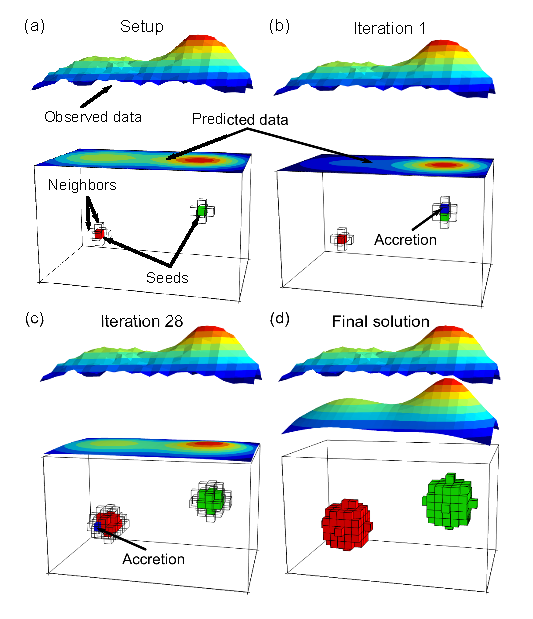
\includegraphics{fig/method}
    \caption{\citet{uieda_animation} provide an animation of this growth
    process.}
    \label{fig:method}
\end{figure}

% APPLICATION
%%%%%%%%%%%%%%%%%%%%%%%%%%%%%%%%%%%%%%%%%%%%%%%%%%%%%%%%%%%%%%%%%%%%%%%%%%%%%%%%
\section{Example application}

\begin{sloppypar}
\end{sloppypar}

% For two-column wide figures use
%\begin{figure*}
% Use the relevant command to insert your figure file.
% For example, with the graphicx package use
  %\includegraphics[width=0.75\textwidth]{example.eps}
% figure caption is below the figure
%\caption{Please write your figure caption here}
%\label{fig:2}       % Give a unique label
%\end{figure*}


% CONCLUSIONS
%%%%%%%%%%%%%%%%%%%%%%%%%%%%%%%%%%%%%%%%%%%%%%%%%%%%%%%%%%%%%%%%%%%%%%%%%%%%%%%%
\section{Conclusions}
\begin{sloppypar}
\end{sloppypar}

% ACKNOWLEDGEMENTS
%%%%%%%%%%%%%%%%%%%%%%%%%%%%%%%%%%%%%%%%%%%%%%%%%%%%%%%%%%%%%%%%%%%%%%%%%%%%%%%%
\begin{acknowledgements}
We acknowledge the use of software
matplotlib by \citet{matplotlib} and
Mayavi by \citet{mayavi}.
The authors were supported in this research by
a fellowship (VCFB) from CNPq
and a scholarship (LU) from CAPES, Brazil.
Additional support for the authors
was provided by the Brazilian agencies
CNPq (grant 471693/2011-1) and FAPERJ (grant E-26/103.175/2011).
\end{acknowledgements}


% REFERENCES
%%%%%%%%%%%%%%%%%%%%%%%%%%%%%%%%%%%%%%%%%%%%%%%%%%%%%%%%%%%%%%%%%%%%%%%%%%%%%%%%
\begin{thebibliography}{}

\bibitem[Cox et~al., 2010]{cox_footprint}
Cox LH, Wilson G a., Zhdanov MS (2010)
3D inversion of airborne electromagnetic data using a moving footprint.
Exploration Geophysics 41:250-259. doi: 10.1071/EG10003

\bibitem[\v{C}uma et~al., 2012]{cuma_largescale}
\v{C}uma M, Wilson G a., Zhdanov MS, Cuma M (2012)
Large-scale 3D inversion of potential field data. Geophysical Prospecting.
doi: 10.1111/j.1365-2478.2011.01052.x

\bibitem[Hunter, 2007]{matplotlib}
Hunter JD (2007)
Matplotlib: A 2D Graphics Environment. Computing in Science \& Engineering
9:90-95. doi: 10.1109/MCSE.2007.55

\bibitem[Last and Kubik, 1983]{last_kubik}
Last BJ, Kubik K (1983)
Compact gravity inversion. Geophysics 48:713-721. doi: 10.1190/1.1441501

\bibitem[Li and Oldenburg, 1998]{li_oldenburg}
Li Y, Oldenburg DW (1998)
3-D inversion of gravity data. Geophysics 63:109-119.
doi: 10.1190/1.1444302

\bibitem[Li and Oldenburg, 2003]{li_compression}
Li Y, Oldenburg DW (2003)
Fast inversion of large-scale magnetic data using wavelet transforms and a
logarithmic barrier method. Geophysical Journal International 152:251-265.
doi: 10.1046/j.1365-246X.2003.01766.x

\bibitem[Martins et~al., 2011]{martins_tv}
Martins CM, Lima WA, Barbosa VCF, Silva JBC (2011)
Total variation regularization for depth-to-basement estimate:
Part 1 - Mathematical details and applications. Geophysics 76:I1-I12.
doi: 10.1190/1.3524286

\bibitem[Ramachandran and Varoquaux, 2011]{mayavi}
Ramachandran P, Varoquaux G (2011)
Mayavi: 3D Visualization of Scientific Data. Computing in Science \& Engineering
13:40-51. doi: 10.1109/MCSE.2011.35

\bibitem[Ren\'e, 1986]{rene}
Ren\'e RM (1986)
Gravity inversion using open, reject, and ``shape-of-anomaly'' fill criteria.
Geophysics 51:988-994. doi: 10.1190/1.1442157

\bibitem[Silva et~al., 2001]{silva_potinversion}
Silva JBC, Medeiros WE, Barbosa VCF (2001)
Potential-field inversion: Choosing the appropriate technique to solve a
geologic problem. Geophysics 66:511-520. doi: 10.1190/1.1444941

\bibitem[Silva and Barbosa, 2006]{silva_interactive}
Silva JBC, Barbosa VCF (2006)
Interactive gravity inversion. Geophysics 71:J1-J9. doi: 10.1190/1.2168010

\bibitem[Silva Dias et~al., 2009]{silvadias_adaptive}
Silva Dias FJS, Barbosa VCF, Silva JBC (2009)
3D gravity inversion through an adaptive-learning procedure.
Geophysics 74:I9-I21. doi: 10.1190/1.3092775

\bibitem[Portniaguine and Zhdanov, 2002]{zhdanov_compression}
Portniaguine O, Zhdanov MS (2002)
3‐D magnetic inversion with data compression and image focusing.
Geophysics 67:1532-1541. doi: 10.1190/1.1512749

\bibitem[Portniaguine and Zhdanov, 1999]{zhdanov_focusing}
Portniaguine O, Zhdanov MS (1999)
Focusing geophysical inversion images. Geophysics 64:874-887.
doi: 10.1190/1.1444596

\bibitem[Uieda and Barbosa, 2012a]{uieda_animation}
Uieda L, Barbosa VCF (2012a)
Animation of growth iterations during 3D gravity gradient inversion by planting
anomalous densities. Figshare. http://dx.doi.org/10.6084/m9.figshare.91469.
Accessed 06 December 2012.

\bibitem[Uieda and Barbosa, 2012b]{uieda_planting}
Uieda L, Barbosa VCF (2012b)
Robust 3D gravity gradient inversion by planting anomalous densities.
Geophysics 77:G55-G66. doi: 10.1190/geo2011-0388.1

\bibitem[Uieda and Barbosa, 2012c]{uieda_shape}
Uieda L, Barbosa VCF (2012c)
Use of the ``shape-of-anomaly'' data misfit in 3D inversion by planting
anomalous densities. SEG Technical Program Expanded Abstracts 2012.
doi: 10.1190/segam2012-0383.1

\end{thebibliography}

\end{document}

